\documentclass[]{article}
\usepackage{booktabs, adjustbox} % Tables
\usepackage{graphicx} % Images graphics
\usepackage{float}    % For floats
\usepackage{siunitx}  % For SI Units
\usepackage{amsmath}  % For multiple math equations
\usepackage{csvsimple}

\graphicspath{{../img/}}



\title{ENPHYS253 \\ Lab 6: Young's Modulus of Steel}
\author{Viraj Bangari \\ 10186046}
\date{\today}

\newcommand{\staticWireDiameter}{\ensuremath{0.52 \pm 0.01 \si{\milli\meter}}}
\newcommand{\staticWireLength}{\ensuremath{2.83 \pm 0.01 \si{\meter}}}
\newcommand{\zero}{\ensuremath{0.170 \pm 0.005 \si{\milli\meter}}}

\newcommand{\Estatic}{\ensuremath{193 \pm 8 \si{\giga\pascal}}}


\newcommand{\slopeIncrease}{\ensuremath{0.697 \pm 0.010 \si{\milli\meter\per\kilo\gram}}}
\newcommand{\slopeDecrease}{\ensuremath{0.679 \pm 0.009 \si{\milli\meter\per\kilo\gram}}}

\newcommand{\slope}{\ensuremath{0.686 \pm 0.007 \si{\milli\meter\per\kilo\gram}}}
\newcommand{\stressMax}{\ensuremath{(9.5 \pm 0.4)*10^{3} \si{\kilo\pascal}}}
\newcommand{\strainMax}{\ensuremath{(2.555 \pm 0.008)*10^{-4}}}

\newcommand{\dynamicWireDiameter}{\ensuremath{(78 \pm 1)*10^{-2} \si{\milli\meter}}}
\newcommand{\dynamicWireLength}{\ensuremath{2.81 \pm 0.01 \si{\meter}}}
\newcommand{\dynamicArea}{\ensuremath{(4.8 \pm 0.1)*10^{-9} \si{\meter^{2}}}}
\newcommand{\M}{\ensuremath{6.949 \pm 0.001\si{\kilo\gram}}}

\newcommand{\freq}{\ensuremath{10.70 \pm 0.01\si{\hertz}}}
\newcommand{\Edynamic}{\ensuremath{(185 \pm 5)*10^{9}\si{\giga\pascal}}}
\newcommand{\sensitivity}{\ensuremath{400\si{\frac{\milli\volt}{g}}}}
\newcommand{\voltage}{\ensuremath{122 \pm 9\si{\milli\volt}}}
\newcommand{\acceleration}{\ensuremath{3.0 \pm 0.2\si{\meter\per\second^2}}}
\newcommand{\Tension}{\ensuremath{89 \pm 2\si{\newton}}}
\newcommand{\stressMaxDynamic}{\ensuremath{(186 \pm 6)*10^{3}\si{\kilo\pascal}}}
\newcommand{\xo}{\ensuremath{(66 \pm 5)*10^{-5}\si{\meter}}}
\newcommand{\strainMaxDynamic}{\ensuremath{(23 \pm 2)*10^{-5}}}
\newcommand{\Q}{\ensuremath{(6.2 \pm 0.2)*10^{2}}}

\begin{document} 
\maketitle

\section{Procedure}
\begin{figure}[H]
    \center
    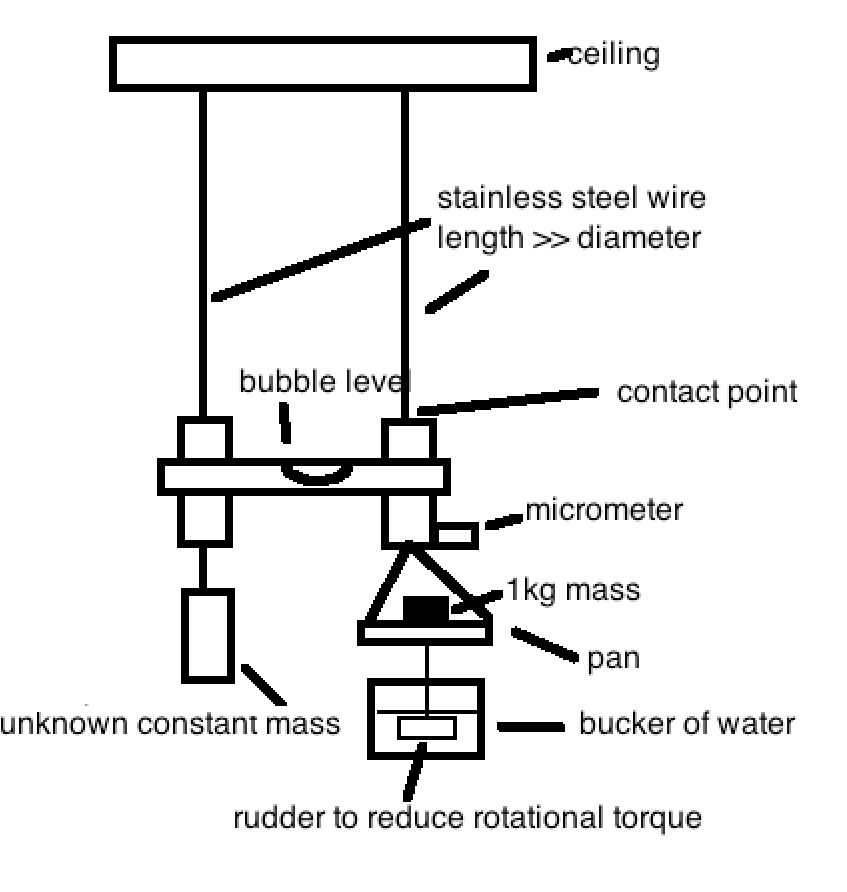
\includegraphics[width=8cm]{../output/diagram1.png}
    \caption{Static Apparatus Diagram}\label{fig:staticapparatus}
\end{figure}
The static apparatus in figure~\ref{fig:staticapparatus} was set up. The
micrometer (each subdivision representing 10 \si{\micro\meter}) was adjusted so
that the bubble level was centered, and the micrometer reading was recorded as
the zero value.  The length of the wire was measured with a two-meter stick by
summing the distances from the halfway point of the wire to the ceiling and to
the and contact point. The length was determined to be \staticWireLength. The
width of the wire was measured by a different micrometer at three points and was
averaged to \staticWireDiameter. A 100 gram weight was added to the pan and the
micrometer was readjusted so that the bubble level was centered. The new
micrometer reading and the added weight (not including the initial kilogram)
were recorded. The change length for the wire is the zero value subtracted from
the micrometer reading.  This process was repeated until the sum of added
weights reached 1000 grams.  Weights were then removed 50 grams at a time until
only the initial 1kg weight was left.  After each removal, the same process of
adjusting the micrometer and recording the measurements was repeated.  The
uncertainty in the weights were considered negligible, and the uncertainty in
the micrometer reading was half the smallest measurement. The largest source of
error was in the bubble level, as there is no way to precisely center it.

\begin{figure}[H]
    \center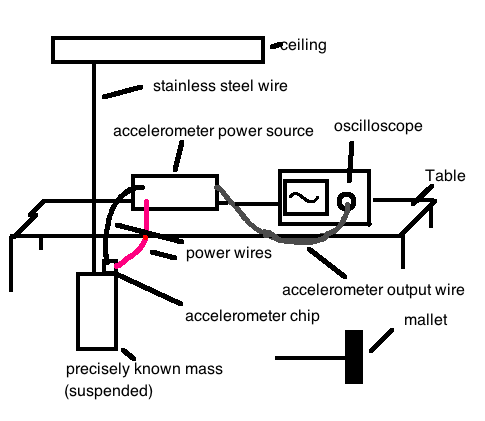
\includegraphics[width=8cm]{../output/diagram2.png}
    \caption{Static Apparatus Diagram}\label{fig:dynamicapparatus}
\end{figure}
The dynamic apparatus in figure~\ref{fig:dynamicapparatus} was set up and the
oscilloscope and accelerometer power source turned on. The accelerometer has a
sensitivity of~\sensitivity. Using the same methods as the static apparatus, the
length of the wire was measured as \dynamicWireLength~and the width was measured
as \dynamicWireDiameter. The power wires in the accelerometer have slack,
allowing that when the mass to oscillate freely. The mass was firmly struck with
the mallet, creating a voltage reading on the oscilloscope. After the
accelerometer readings had stabilized into a simple harmonic waveform, the
oscilloscope signal was frozen. The horizontal cursors in the oscilloscope were
used to measure the pk-pk voltage amplitude of the wave, and the vertical
cursors were used to measure the time between ten full periods.  The voltage and
time readings were recorded. This process was repeated two more times. The mass
was struck again, but the oscilloscope was frozen after the reading had started
damping. The horizontal cursors were used to find the points where the pk-pk
amplitudes had dampened by a factor of one half, and the vertical cursors were
used to find the time difference. The time difference was recorded.  This
process was repeated two more times for the same change in amplitude.  Since the
voltage and time measurements were taken multiple times, their uncertainty is
their standard error of the mean.

\section{Results and Analysis}
The static apparatus load data from table~\ref{tab:increasing} and
table~\ref{tab:decreasing} was plotted onto figure~\ref{fig:static} and a linear
regression was performed.  The slopes were determined to be \slopeIncrease~and
\slopeDecrease, which are identical within experimental error. Residual plots
were created on figures~\ref{fig:decreaseresidual}
and~\ref{fig:increaseresidual}, with both having no discernible pattern. The two
datasets were combined and plotted onto figure~\ref{fig:combined}, while the
residuals were plotted onto figure~\ref{fig:combinedresidual}. The slope from
the linear regression was determined to be~\slope. This slope was used with
equation~\ref{eq:Estatic} to calculate the Young's modulus of the stainless
steel wire as~\Estatic, agreeing with the accepted range of Young's modulus of
stainless steel of $180 \si{\giga\pascal}$ to $200
\si{\giga\pascal}$\cite{ref:young}. Using the second-last data point in
table~\ref{tab:increasing} with equation~\ref{eq:Estatic}, the maximum stress
was calculated as~\stressMax~and the maximum strain was calculated
as~\strainMax.

The dynamic apparatus time data from table~\ref{tab:dynamic} was used to
calculate the average frequency of oscillate as~\freq. This frequency was used with
equation~\ref{eq:Edynamic} to determine the Young's modulus for stainless steel
as~\Edynamic. This value also lies within the expected range of $180
\si{\giga\pascal}$ to $200 \si{\giga\pascal}$\cite{ref:young}. By calculating
the average voltage as while knowing that the chip sensitivity was~\sensitivity, the
maximum acceleration of the mass was calculated as~\acceleration. From
equation~\ref{eq:Tension}, it was determined that the maximum tension in the
wire occurred when the magnitude of the acceleration was at a maximum and its
direction opposed gravity. The maximum tension was calculated as~\Tension,
resulting in a maximum stress of \stressMaxDynamic. The maximum acceleration was
used with equation~\ref{eq:oscillation} to determine the amplitude of
vibration $x_o$. Since the acceleration was a maximum, the cosine term in
equation~\ref{eq:oscillation}~equalled 1, making it possible the amplitude of
vibration as \xo.  Knowing that the maximum strain occurs at $x_o$, it was
calculated as \strainMaxDynamic. The times it took for the amplitude to decrease
by a factor of 0.5 from table~\ref{tab:half} was averaged and used with
equation~\ref{eq:Q} in order to calculate the quality factor as \Q.


\newpage
% Part 1
\begin{figure}[H]
    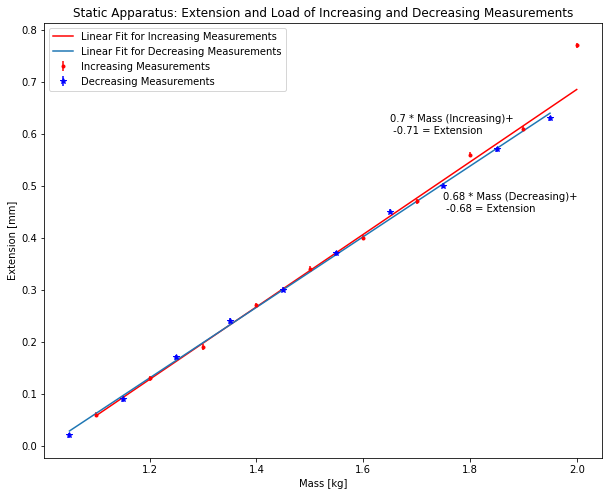
\includegraphics[width=\textwidth]{../output/staticgraph.png}
    \caption{Static Apparatus: Extension and Load of Increasing and Decreasing
    Measurements with stainless steel wire length \staticWireLength~and diameter
    \staticWireDiameter}\label{fig:static}
    Note: The last data point in the increasing loads was ignored from the
    linear fit and subsequent plots/calculations as it appears as an outlier.
\end{figure}

\begin{figure}[H]
    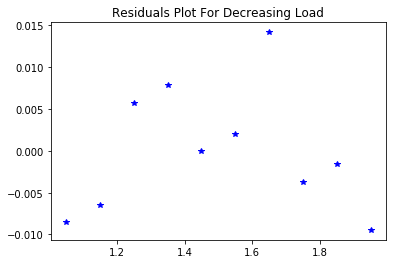
\includegraphics[width=\textwidth]{../output/residualsdecrease.png}
    \caption{Residuals Plot For Increasing Load}\label{fig:decreaseresidual}
\end{figure}

\begin{figure}[H]
    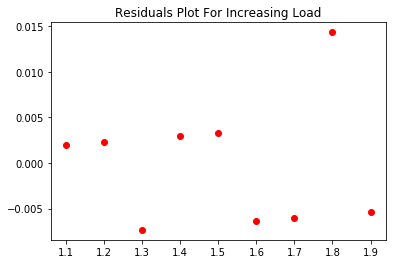
\includegraphics[width=\textwidth]{../output/residualsincrease.png}
    \caption{Residuals Plot For Decreasing Load}\label{fig:increaseresidual}
\end{figure}

\begin{figure}[H]
    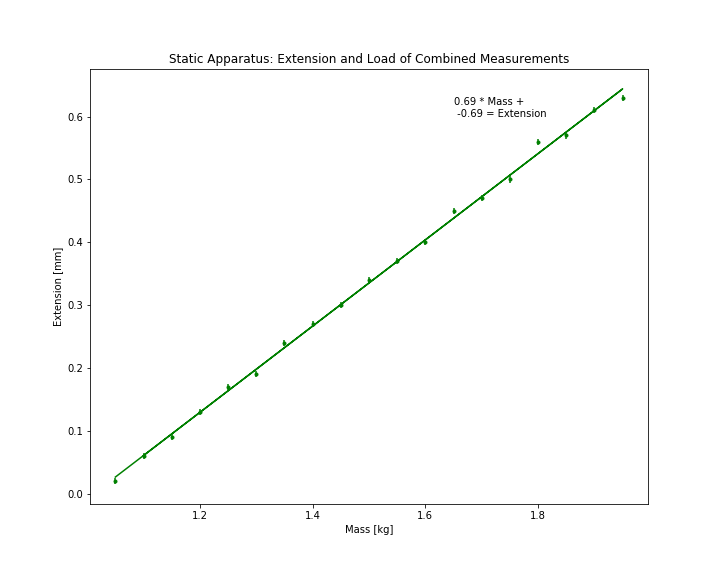
\includegraphics[width=\textwidth]{../output/combinedstaticgraph.png}
    \caption{Static Apparatus: Extension and Load of Increasing and Decreasing
    Measurements with stainless steel wire length \staticWireLength and diameter
    \staticWireDiameter}\label{fig:combined}
\end{figure}

\begin{figure}[H]
    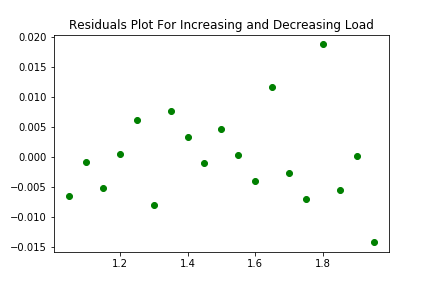
\includegraphics[width=\textwidth]{../output/residualscombined.png}
    \caption{Residuals Plot For Increasing and Decreasing Load}\label{fig:combinedresidual}
\end{figure}

\newpage
\section{Appendix}
\subsection{Equation List} 
\subsubsection{Static Case}
\begin{equation}\label{eq:Estatic}
    E = \frac{stress}{strain} = \frac{F l}{A \Delta l} = \frac{mgl}{A\Delta l}
\end{equation}
$E$ is Young's modulus, $F$ is the tensile force acting over the cross sectional
area $A$, $l$ is the length, $\Delta l$ is the change in length, $m$ is mass and
$g$ is gravitational acceleration.

\subsubsection{Dynamic Case}
$T$ is the tension in the wire. These are the forces acting upon the mass.
\begin{equation}\label{eq:Edynamic}
    E = {(2\pi f_{avg})}^2 Ml/A
\end{equation}
$f_{avg}$ is the frequency of oscillation, $M$ is the mass.

\begin{equation}\label{eq:Tension}
    M\ddot{x} = T - Mg
\end{equation}
$\ddot{x}$ is the acceleration of the mass, $T$ is the tension in the wire. These
are the forces acting upon the mass.

\begin{equation}\label{eq:oscillation}
    \ddot{x} = -{(2\pi f)}^2 x_o \cos(2\pi ft + \phi)
\end{equation}
$t$ is time, $x_o$ is the amplitude of vibration.

\begin{equation}\label{eq:Q}
    Q = \pi t_{1/2}f/\ln(2)
\end{equation}
$Q$ is the quality factor, $t_{1/2}$ is time for the amplitude to decay by a
factor of 1/2.

\subsection{Raw Data}

\begin{table}[H]
    \centering
    \caption{Extension for Increasing Loads in Static Apparatus with Stainless
    Steel Wire with Length \staticWireLength, Diameter \staticWireDiameter~and
    Zeroed Extension at \zero}\label{tab:increasing}
    \begin{tabular}{@{}cc@{}}
        \toprule
        Mass (kg) & Micrometer Extension {[}mm{]} +/- 0.005 [mm] \\ \midrule
        0.1       & 0.23                                    \\
        0.2       & 0.3                                     \\
        0.3       & 0.36                                    \\
        0.4       & 0.44                                    \\
        0.5       & 0.51                                    \\
        0.6       & 0.57                                    \\
        0.7       & 0.64                                    \\
        0.8       & 0.73                                    \\
        0.9       & 0.78                                    \\
        1         & 0.94                                    \\ \bottomrule
    \end{tabular}
\end{table}

\begin{table}[H]
    \centering
    \caption{Extension for Decreasing Loads in Static Apparatus with Stainless
    Steel Wire with Length \staticWireLength, Diameter \staticWireDiameter~and
    Zeroed Extension at \zero}\label{tab:decreasing}
    \begin{tabular}{@{}cc@{}}
        \toprule
        Mass (kg) & Micrometer Extension {[}mm{]} +/- 0.005 {[}mm{]} \\ \midrule
        0.95      & 0.8                                              \\
        0.85      & 0.74                                             \\
        0.75      & 0.67                                             \\
        0.65      & 0.62                                             \\
        0.55      & 0.54                                             \\
        0.45      & 0.47                                             \\
        0.35      & 0.41                                             \\
        0.25      & 0.34                                             \\
        0.15      & 0.26                                             \\
        0.05      & 0.19                                             \\ \bottomrule
    \end{tabular}
\end{table}

\begin{table}[H]
    \centering
    \caption{Time for 10 Periods of Dynamic Apparatus with Stainless
    Steel Wire with Length \dynamicWireLength, Diameter \dynamicWireDiameter,
    mass \M~and voltage sensitivity~\sensitivity}\label{tab:dynamic}
    \begin{tabular}{@{}ll@{}}
        \toprule
        Time {[}ms{]} & Amplitude {[}mV{]} \\ \midrule
        936           & 248                \\
        934           & 250                \\
        934           & 232                \\ \bottomrule
    \end{tabular}
\end{table}

\begin{table}[H]
    \centering
    \caption{Time for Amplitude to go from $140\si{\milli\volt}$ to
    $70\si{\milli\volt}$ with Stainless Steel Wire with Length
    \dynamicWireLength, Diameter \dynamicWireDiameter, mass \M~and voltage
    sensitivity~\sensitivity}\label{tab:half}
    \begin{tabular}{@{}l@{}}
        \toprule
        Time {[}s{]} +/- 0.5 {[}s{]} \\ \midrule
        12.9                         \\
        12                           \\
        12.97                        \\
        12.16                        \\
        14.16                        \\ \bottomrule
    \end{tabular}
\end{table}

\subsection{Sample Calculations}
\subsubsection{Young's Modulus (Static)}
Using equation~\ref{eq:Estatic} and the slope from~\ref{fig:combined}, the
following equation can be used: ${(\frac{slope}{g})}^{-1} \frac{l}{A}$\\

$= \frac{(\staticWireLength/9.81)^{-1}*\staticWireLength}{\pi{(\staticWireDiameter/2)}^2} $

$= \Estatic$


\subsubsection{Maximum Stress (Static)}
Stress $ = F_{\max}/A$

$= (2 kg * 9.81 m/s^2)/\pi{(\staticWireDiameter/2)}^2$

$= \stressMax$

\subsubsection{Maximum Strain (Static)}
$\Delta l/l$

$2.155*10^4/\staticWireLength$

Strain$= \strainMax$

\subsubsection{Young's Modulus (Dynamic)}
$E = {(2\pi f_{avg})}^2 Ml/A$

$= {(2\pi \freq)}^2 \M\dynamicWireLength/\dynamicArea$

$= \Edynamic$

\subsubsection{Maximum Acceleration (Dynamic)}
$\ddot{x}_{\max} = 1/\sensitivity * V_{avg} * 9.81\si{\meter\per\second^2}$

$= 1/\sensitivity * \voltage * 9.81\si{\meter\per\second^2}$

$= \acceleration$

\subsubsection{Maximum Stress (Dynamic)}
Stress = $T/A$

$= M(a + g)/A$

$= \M(\acceleration + 9.81\si{\meter\per\second^2})/\dynamicArea$

$= \stressMaxDynamic$

\subsubsection{Amplitude of Vibration (Dynamic)}
$\ddot{x}_{\max} = -{(2\pi f)}^2 x_o \cos(2\pi ft + \phi)$

$x_o = \ddot{x}/{(2\pi f)}^2$

$x_o = \acceleration/{(2\pi \freq)}^2$

$x_o = \xo$

\subsubsection{Maximum Strain (Dynamic)}
Strain = $x/l$

$= \xo/\dynamicWireLength$

$= \M(\acceleration + 9.81\si{\meter\per\second^2})/\dynamicArea$

$= \strainMaxDynamic$
\bibliographystyle{ieeetr}
\bibliography{lab6}
\end{document}
